\chapter{Revisão Teórica}
\label{cap:teo}

Neste capítulo, introduziremos brevemente a base do pensamento modal. 

A lógica modal é determinada semanticamente pela avaliação de necessidade e
possibilidade de uma proposição, levando em consideração diferentes possíveis
contextos (ou \emph{mundos}). Na literatura, representações análogas à de
necessidade e possibilidade são utilizadas para a avaliação de estados
epistemológicos, como por exemplo, conhecimento e crença,
respectivamente~\cite{belief}. Basicamente, uma proposição é \textit{necessária}
se ocorre em todos os mundos possíveis e \textit{possível} se ocorre em algum
mundo~\cite{chellas:modal_logic}.  A ideia é que uma ação ou objeto pode
possuir valorações distintas em mundos diferentes, mas qualquer objeto que
possuir valoração verdadeira em todos os mundos possíveis é necessária, enquanto
a que ocorre em pelo menos um mundo, é possível.

Os operadores utilizados são os mesmos já conhecidos da lógica proposicional
($\wedge$, $\vee$, $\rightarrow$ etc) com a inclusão de dois novos:
$\nec{\agent}$ e $\pos{\agent}$. Uma sentença da forma $\nec{\agent} \varphi$
(\textit{necessariamente} $\varphi$) é verdadeira se, e somente se, $\varphi$ é
uma proposição verdadeira em todos os mundos possíveis, de acordo com o agente
$\agent$; já uma sentença da forma $\pos{\agent} \varphi$
(\textit{possivelmente} $\varphi$) é verdadeira no caso em que $\varphi$ é uma
proposição verdadeira em algum mundo existente, também de acordo com o agente
$\agent$.

Uma ilustração válida para a lógica modal, é pensar em uma coleção de possíveis
mundos, incluindo nosso próprio, o mundo real, onde sentenças da linguagem são
possivelmente verdadeiras ou falsas. O propósito principal da lógica modal é
modelar a ocorrência verdadeira destas sentenças. Esta lógica pode ser expressa
de diferentes formas e contar com diferentes axiomas. %através da ideia de
%sistemas, isto será explorado com mais detalhes 
%na seção~\ref{sec:sistemas}. 

\section{Lógica}
\label{sec:logicas}

A lógica permite chegar a uma conclusão (ou mais de uma conclusão) a partir de
um conjunto de premissas (ou hipóteses), isto é, lógica expressa raciocínio. É
necessário entender claramente o que é lógica e por que seu estudo é importante
(e difícil), portanto, esta seção é dedicada a este fim. Nesta seção são
apresentadas algumas definições importantes que são centrais no estudo da
lógica.

Lógica é a análise e a avaliação de argumentos~\cite{gensler}, é a tentativa de
se separar linhas de raciocínios viáveis das inviáveis. É possível definir
raciocínio sobre qualquer tópico, tanto filosófico (por exemplo livre arbitrio e
determinismo, existência de um deus, moralidade etc) como não-filosófico (por
exemplo poluição, futebol, construção de um arranha-céu etc). Sendo assim, a
lógica é uma ferramenta muito útil no raciocínio tanto de questões com um
significado mais profundo, quanto em questões do dia a dia.

Pode-se pensar em três principais justificativas para o estudo de lógica.
Primeiro, é difícil imaginar uma tomada de decisão ou a chegada a uma conclusão,
uma resposta a alguma pergunta, sem pensar que houve uma linha de raciocínio
envolvida, portanto raciocínio é importante. Raciocínio e habilidades analíticas
em geral são fundamentais nas mais diversas áreas. Observe, então, que a lógica
é importante pois seu estudo é a tentativa de compreensão e evolução do
raciocínio. Segundo, a lógica pode aprofundar conhecimentos filosóficos. Sem
lógica, um indivíduo pode apenas divagar de forma vaga sobre as questões de vida
que a filosofia levanta, ou seja, há ausência de suporte ferramental para
compreender e avaliar raciocínios desta natureza. Finalmente, lógica pode ser
bastante divertido. Ela desafia o pensamento a seguir caminhos novos e realizar
processos diferentes, como a montagem de um quebra-cabeça.

A Figura~\ref{fig:exemplo_rac} mostra um exemplo de problema sobre o qual
é possível raciocinar usando lógica.

\begin{figure}[!tbh]
\label{fig:exemplo_rac}
\begin{center}
    \begin{tabular}{cc}
        Caso 1 & Caso 2 \\
        \begin{tabular}{|c|}
            \hline
            Se o cachorro latir, o bebê vai acordar. \\
            O bebê não acordou.\\
            \hline
        \end{tabular}
        &
        \begin{tabular}{|c|}
            \hline
            Se o cachorro latir, o bebê vai acordar. \\
            O cachorro não latiu.\\
            \hline
        \end{tabular}
    \end{tabular}
\end{center}
    \caption{Exemplo de problema sobre o qual se pode raciocinar}
\end{figure}

No primeiro caso, a conclusão de que o cachorro não latiu é trivial. Já no
segundo caso, algumas pessoas se sentiriam tentadas a concluir que o bebê não
acordou, o que não é necessariamente verdade, já que o bebê poderia ter acordado
com outros ruídos ou por estar com fome, por exemplo. A intuição lógica pode ser
trabalhada com a finalidade de servir como ferramenta de raciocínio sobre
argumentos. Por se tratar de um conhecimento acumulativo, quanto mais
aprofundado o estudo de lógica, mais precisa se torna esta ferramenta.

\begin{definition}
   Um \textbf{argumento}, no sentido usado em lógica, é um conjunto de
   afirmações consistindo em premissas e uma conclusão. As \textbf{premissas}
   são afirmações de partida, ou hipóteses, que dão suporte a uma evidência; o
   que estas hipóteses evidenciam é definido como \textbf{conclusão}.
\end{definition}

No exemplo da Figura~\ref{fig:exemplo_arg}, as duas primeiras linhas representam
as premissas do argumento e a última linha é a conclusão.

\begin{figure}[!tbh]
\label{fig:exemplo_arg}
\begin{center}
        \begin{tabular}{|l|}
            \hline
            Se o cachorro latir, o bebê vai acordar. \\
            O bebê não acordou.\\
            Portanto, o cachorro não latiu.\\
            \hline
        \end{tabular}
\end{center}
    \caption{Exemplo de argumento}
\end{figure}

A definição a seguir representa uma primeira noção de um argumento
\textbf{válido}, no contexto de lógica.

\begin{definition}
   Um argumento é \textbf{válido} quando for impossível ou contraditório ter
   todas as premissas verdadeiras e a conclusão falsa.
\end{definition}

O que se quer dizer com essa definição é apenas que, em um argumento válido, a
conclusão \textit{segue} das premissas~\cite{gensler}, ou seja, se as premissas
forem todas verdadeiras, então a conclusão também é.
A Figura~\ref{fig:exemplo_arg} representa um exemplo de argumento válido,
enquanto a Figura~\ref{fig:exemplo_arg_invalido} representa um exemplo de
argumento inválido, como visto anteriormente.

\begin{figure}[!tbh]
\label{fig:exemplo_arg_invalido}
\begin{center}
        \begin{tabular}{|l|}
            \hline
            Se o cachorro latir, o bebê vai acordar. \\
            O cachorro não latiu.\\
            Portanto, o bebê não acordou.\\
            \hline
        \end{tabular}
\end{center}
    \caption{Exemplo de argumento inválido}
\end{figure}

Estas definições iniciais são apenas alguns passos na direção da compreensão da
ideia geral que a lógica trata. Lógica requer estudos cuidadosos, possui 
tópicos difíceis além de parcialmente abstratos.


\subsection{Linguagens Lógicas}
\label{sec:linguagens}
Uma linguagem lógica é uma formalização.  Nesse sentido, é possível definir
diversas linguagens lógicas que podem diferir em modalidades de aplicabilidade,
expressividade e complexidade, por exemplo. A linguagem foco deste trabalho é a
Linguagem Modal \system{K}{n}{}. Esta seção tem o objetivo de apresentar
teoricamente, e de forma abstrata, uma visão geral desta linguagem, que será
construída a partir de linguagens menos expressivas, já apresentadas com a noção
de mundos possíveis, muito utilizada na lógica modal.

%Lógica proposicional
É bastante usual que as pessoas tenham contato com lógica em algum momento da
vida. Este contato é, em geral, com a Lógica Proposicional Básica.
Esta lógica estuda argumentos cuja validade depende das noções de ``se-então'',
``e'', ``ou'', ``não'', além de noções similares. Estas noções definem os
operadores mais usuais da lógica. 

A Linguagem Proposicional é, portanto, uma formalização que provê regras
específicas para construção de argumentos e testes de validade que utilizam
estas noções~\cite{gensler}. A especificação apresentada neste documento,
utiliza consoantes minúsculas para representar afirmações at\^omicas, ou seja,
uma proposição que pode ser verdadeira ou falsa. Os operadores utilizados estão
expressos na Tabela~\ref{tab:operadores_prop}.

\begin{table}[!tbh]
\label{tab:operadores_prop}
\caption{Operadores da Lógica Proposicional}
\begin{center}
\begin{tabular}{|rcl|}
   \hline  
   $\neg p$ & $:=$ & $\text{não}\ p$ \\
   $p \wedge q$ & $:=$ & $p\ \text{e}\ q$ \\
   $p \vee q$ & $:=$ & $p\ \text{ou}\ q$ \\
   $p \then q$ & $:=$ & se $p$ então $q$ \\
   $p \iff q$ & $:=$ & $p$ se, e somente se, $q$ \\
   \hline
\end{tabular}
\end{center}
\end{table}

Os operadores podem ser combinados entre si e com símbolos at\^omicos (ou
proposicionais) para formar fórmulas. As fórmulas que pertencem a Linguagem
Proposicional, são as bem formadas, ou seja, que expressam um significado, como
definido a seguir:

\begin{definition}
   As fórmulas bem formadas da Linguagem Proposicional são definidas
   recursivamente como segue:
   \begin{itemize}
       \item [(i)] Os símbolos proposicionais $(p,q,\ldots)$ são fórmulas bem formadas
   \end{itemize}
   Agora considere que $\varphi$ e $\psi$ são fórmulas bem formadas. Então:
   \begin{itemize}
       \item [(ii)] $\neg \varphi$
       \item [(iii)] $\varphi \wedge \psi$
       \item [(iv)] $\varphi \vee \psi$
       \item [(v)] $\varphi \then \psi$
       \item [(vi)] $\varphi \iff \psi$
   \end{itemize}
   também são fórmulas bem formadas.
\end{definition}

Observe que é possível representar equivalências entre os operadores, conforme
exemplos na Tabela~\ref{tab:equivalencia}.  Neste sentido, os operadores $\neg$
e $\vee$ são suficientes para expressar toda a Lógica Proposicional. Os demais
são utilizados para facilitar a leitura e diminuir o tamanho das fórmulas.

\begin{table}[!h]
\label{tab:equivalencia}
\caption{Equivalência entre operadores}
\begin{center}
\begin{tabular}{|rcl|}
   \hline  
   $\neg (p \vee q)$ & $=$ & $\neg p \wedge \neg q$ \\
   $p \then q$ & $=$ & $\neg p \vee q$ \\
   $p \iff q$ & $=$ & $(p \then q) \wedge (q \then p)$ \\
   \hline
\end{tabular}
\end{center}
\end{table}

Agora já podemos começar a raciocinar sobre algum mundo possível utilizando
Lógica Proposicional. 

Seja, então, $t$ o planeta em que vivemos. É possível escrever diversas
afirmações que podem ter valoração verdadeira ou falsa e é possível combiná-las
para escrever argumentos. Considere as afirmações contidas na
Figura~\ref{fig:prop}.

\begin{figure}[!tbh]
\label{fig:prop}
\begin{center}
\begin{tabular}{|l|}
   \hline  
   $p:$ O céu é azul.\\
   $r:$ O Brasil fica na América do Sul.\\
   $s:$ Machado de Assis nasceu no Brasil.\\
   $v:$ Machado de Assis nasceu na América do Sul.\\
   $z:$ A Argentina fica na Ásia.\\
   $q:$ Buenos Aires é a capital da Argentina.\\
   $l:$ Buenos Aires fica na Ásia.\\
   \hline
\end{tabular}
\end{center}
\caption{Exemplos de afirmações sobre o nosso planeta}
\end{figure}

Sabemos que $p,r,s,v$ e $q$ são verdadeiras e que $z$ e $l$ são falsas. Observe
os argumentos descritos na Figura~\ref{fig:argumentos_prop}. 

\begin{figure}[!tbh]
\label{fig:argumentos_prop}
\begin{center}
    \begin{tabular}{ccc}
        \begin{tabular}{|r|}
            \hline
            Premissas:\\
            $r$\\
            $s$\\
            \hline
            Conclusão:\\
            $v$\\
            \hline
        \end{tabular}
        &
        \begin{tabular}{|r|}
            \hline
            Premissas:\\
            $p$\\
            $q$\\
            \hline
            Conclusão:\\
            $z$\\
            \hline
        \end{tabular}
        &
        \begin{tabular}{|r|}
            \hline
            Premissas:\\
            $z$\\
            $q$\\
            \hline
            Conclusão:\\
            $l$\\
            \hline
        \end{tabular} \\
        (a) & (b) & (c)
    \end{tabular}
\end{center}
\caption{Exemplos de argumentos sobre as afirmações da Figura~\ref{fig:prop}}
\end{figure}

Conforme a definição de validade vista no começo desta seção, podemos concluir
que (a) e (c) são argumentos válidos, e (b) é um argumento inválido. Vale
lembrar que estes argumentos estão definidos no Planeta Terra ($t$), então
podemos esboçar um modelo que satisfaz os argumentos válidos, conforme
Figura~\ref{fig:modelos_prop}.

\begin{center}
\begin{figure}
\label{fig:modelos_prop}
\begin{center}
\begin{tabular}{cc}
\begin{tikzpicture}
\matrix[nodes={draw,thick, minimum size=1.5cm},
row sep=0.3cm,column sep=1.5cm,ampersand replacement=\&] {
    \node[circle,label=150:$t$](w0) {$
        \begin{array}{c}       
            r\quad s\\
            v
        \end{array}
    $}; \\
};

\end{tikzpicture}
&
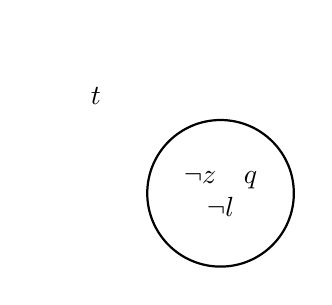
\begin{tikzpicture}
\matrix[nodes={draw,thick, minimum size=1.5cm},
row sep=0.3cm,column sep=1.5cm,ampersand replacement=\&] {
    \node[circle,label=150:$t$](w0) {$
        \begin{array}{c}       
            \neg z\quad q\\
            \neg l
        \end{array}
    $}; \\
};

\end{tikzpicture} \\
(a) & (c)
\end{tabular}
\end{center}
\caption{Modelos que satisfazem os argumentos (a) e (c) da
Figure~\ref{fig:argumentos_prop}}
\end{figure}
\end{center}

FAZER O LINK DE ARGUMENTOS PARA FÓRMULAS



%Lógica modal um agente
Na Lógica Proposicional, existe apenas um contexto no qual se pode raciocinar.
Se uma proposição é verdadeira, não é possível que ela seja falsa. Podemos
estender a noção estudada nesta lógica para uma visão mais ampla, que dependa
dos contextos que se é possível enxergar, ou seja, raciocinar sobre, aumentando o
poder de expressividade da linguagem vista anteriormente. A Lógica Modal define
uma dessas possíveis extensões.

Além das noções expressas através dos operadores proposicionais, a Lógica Modal
estuda argumentos cuja validade depende das noções de ``necessidade'' e
``possibilidade'' (representações análogas são possíveis e foram citadas no
início deste capítulo). Estas noções dizem respeito a valoração das proposições
em diferentes contextos. A notação utilizada para representar estes dois novos
operadores e suas respectivas semânticas na Linguagem Modal estão expressas na Tabela~\ref{tab:op_modal}.

\begin{table}[!h]
    \label{tab:op_modal}
    \caption{Operadores Modais}
\begin{center}
    \begin{tabular}{|rcl|}
       \hline 
       $\pos{} p$ & $:=$ & $p$ é possível, ou seja, $p$ é verdadeiro em algum mundo
       possível\\
       $\nec{} p$ & $:=$ & $p$ é necessário, ou seja, $p$ é verdadeiro em todos os mundos
       possíveis\\
       \hline
    \end{tabular}
\end{center}
\end{table}

As regras de formação de fórmulas são as mesmas da Linguagem Proposicional, com
a seguinte extensão para cobrir os operadores modais:

\begin{definition}
   Se $\varphi$ é uma fórmula bem formada então:
   \begin{itemize}
       \item [$(vii)$] $\pos{} \varphi$ 
       \item [$(viii)$] $\nec{} \varphi$ 
   \end{itemize}
   também são fórmulas bem formadas.
\end{definition}


%Lógica multimodal

\section{Formalização da Linguagem Modal \system{K}{n}{}}
Definições formais podem ser úteis ao entendimento.
Esta seção é dedicada a trazer o básico dos conceitos de sintaxe e semântica da linguagem da
lógica modal. 

\subsection{Sintaxe}
\label{sec:sintaxe}

A linguagem proposicional clássica é formada por um conjunto enumerável de sentenças
\textit{at\^omicas} (ou símbolos proposicionais): 
\begin{equation}
\label{simb_prop}
    \mathcal{P} = \{p, q, r, \ldots\}
\end{equation}
Estas são as sentenças mais simples possível.

Já as \textit{sentenças moleculares} (não-at\^omicas) são formadas por meio das
\textit{operações sintáticas}, ou \textit{operadores lógicos} de negação
($\neg$), de disjunção ($\vee$)  e de necessidade ($\nec{\agent}$, para todo
$\agent \in \Agents = \{1,\ldots, n\}$, $n \in \Nat$). Observe que $\neg$ e
$\nec{\agent}$ são operadores unários e $\vee$ é um operador binário. Além
disso, um conjunto de sinais de pontuação $\{(,)\}$ é usado para
evitar ambiguidade na leitura de sentenças.

Podemos então definir uma fórmula como uma combinação finita de sentenças
moleculares. A \textit{Linguagem Lógica Modal} é, portanto, equivalente ao seu
conjunto de \textit{fórmulas bem formadas}, definido a seguir.

\begin{definition} O conjunto de \textit{fórmulas bem formadas da linguagem modal}, denotado por
$FBF_{K}$ é definido indutivamente como segue:
    \label{def:fbf}

    \begin{enumerate}
    \item Os símbolos proposicionais estão em $FBF_{K}$;
    \item Se $\varphi \in FBF_{K}$, então $\neg \varphi$ e $\nec{\agent}\varphi$, $\agent \in \Agents$, estão em $FBF_{K}$; e
    \item Se $\varphi$ e $\psi$ estão em $FBF_{K}$, então $(\varphi \vee \psi)$ está em $FBF_{K}$.
    \end{enumerate}
    
\label{def:fbf}
\end{definition}

Outros operadores lógicos podem ser introduzidos como abreviações para fórmulas
construídas a partir dos operadores já definidos, como usual. Em particular,
neste trabalho as seguintes abreviações serão utilizadas: $(\varphi \land \psi)
= \neg (\neg \varphi \lor \neg \psi)$ (conjunção), $(\varphi \then \psi) = (\neg
\varphi \lor \psi)$ (implicação), $\pos{\agent} \varphi= \neg \nec{\agent} \neg
\varphi$ (possibilidade), $\cfalse = (\varphi \land \neg \varphi)$
(\emph{falsum}) e $\ctrue = \neg \cfalse$ (\emph{verum}). A precedência dos
operadores é dada na seguinte ordem (onde $\agent \in \Agents)$:
\begin{enumerate} 
    \item $\{\neg, \nec{\agent}, \pos{\agent}\}$ 
    \item $\{\wedge\}$ 
    \item $\{\vee\}$ 
    \item $\{\rightarrow\}$ 
\end{enumerate}

Quando não houver ambiguidade na leitura de uma fórmula, parênteses podem ser
omitidos.

Lógicas que envolvem vários agentes na lógica modal utilizam $n$ operadores, com
$n \in \mathbb{N}$, como descrito acima, são chamadas de \emph{lógicas
multimodais}. A lógica modal com um único agente, onde apenas temos os
operadores $\pos{1}$ e $\nec{1}$ (ou simplesmente $\pos{}$ e $\nec{}$), isto é,
onde $\Agents =\{1\}$, bem como a lógica proposicional clássica, onde $\Agents =
\{\}$, são, portanto, casos especiais da lógica multimodal.

O \emph{nível modal} de uma fórmula é o número máximo de ocorrências de
operadores modais sob o qual a fórmula ocorre. Por exemplo, em
$\nec{\agent}\pos{\agent}p$, o nível modal de $p$ é 2.

É importante definir algumas convenções para minimizar 
dúvidas que poderiam surgir em algumas expressões.
Expressões da forma $A_1 \wedge \ldots \wedge A_n$ e $A_1 \vee \ldots \vee A_n$
representam conjunções e disjunções arbitrárias mas não especificadas das
sentenças $A_1,\ldots,A_n$. O objetivo é deixar claro que tanto $\wedge$ como
$\vee$ obedecem as regras de associatividade lógica. 

\subsection{Semântica}
\label{semantics}

A ideia geral do significado de fórmulas na lógica proposicional modal pode ser
entendida, de forma simples, em termos de uma coleção de mundos possíveis, um conjunto
de atribuições de valores booleanos para cada símbolo proposicional em cada
mundo e relações de acessibilidade, que são definidas com base em um conjunto de
agentes.

Uma das estruturas mais estudadas em lógica modal corresponde à estrutura de
Kripke. 

\begin{definition}
    Uma \textbf{estrutura de Kripke}, para o conjunto de símbolos proposicionais
    $\mathcal{P}$ e o conjunto de agentes $\Agents = \{1,\ldots, n\}$, é
    uma tupla $\mathcal{M} = (W, \st_0, R_1,\ldots, R_n, \pi)$, onde:
   $W$ é um conjunto não-vazio de mundos possíveis; $\st_0 \in W$ é a raiz do modelo; 
   $\forall\agent \in \Agents, R_\agent \subseteq W \times W$ e
   $\pi : W \times \mathcal{P} \longrightarrow \{false, true\}$
    
\end{definition}

A partir da definição de estrutura de Kripke, podemos definir a satisfatibilidade
e a validade de uma fórmula.
\begin{definition}
    Seja $\mathcal{M} = (W, \st_0, R_1, \ldots, R_n, \pi)$ uma estrutura de Kripke sobre
    $\mathcal{P}$ e $\Agents$, e considere $w \in W$, $p \in \mathcal{P}$
    e $\varphi$ e $\psi$ fórmulas bem formadas. A \textbf{relação de
    satisfatibilidade}, denotada por $\models ^{\mathcal{M}}_{w} \varphi$, entre
    o mundo $w$ e uma fórmula $\varphi$ no modelo $\mathcal{M}$, é definida
    indutivamente como se segue:
    \begin{itemize}
        \item $\models ^{\mathcal{M}}_{w} p$ se e somente se, $\pi(w,p) =
            true$;
        %\item $\models ^{\mathcal{M}}_{w} true$ e $\not\models ^{\mathcal{M}}_{w} false$; Você não precisa disso. Falso e verdateiro são abreviações.
        \item $\models ^{\mathcal{M}}_{w} \neg \varphi$ se e somente se,
            $\not\models ^{\mathcal{M}}_{w} \varphi$
            
        \item $\models ^{\mathcal{M}}_{w} \varphi \vee \psi$ se e somente se,
            $\models ^{\mathcal{M}}_{w} \varphi$ \texttt{ou} $\models
            ^{\mathcal{M}}_{w} \psi$
        \item $\models ^{\mathcal{M}}_{w} \nec{\agent} \varphi$ se e somente se,
            $\forall~t \in W$ com $\agent \in \Agents$  e $(w,t) \in R_\agent$,
            tem-se que $\models ^{\mathcal{M}}_{t} \varphi$. 
    \end{itemize}
\end{definition}

\begin{definition}
    Seja $\varphi \in FBF_{K}$, dizemos que $\varphi$ é
    \textbf{satisfatível} se existe um modelo $\mathcal{M}$ tal que $\models ^{\mathcal{M}}_{\st_0} \varphi$.  
\end{definition}

\begin{definition}
    Seja $\varphi \in FBF_{K}$, dizemos que $\varphi$ é
    \textbf{válida} se para todo modelo $\mathcal{M}$ temos que $\models ^{\mathcal{M}}_{\st_0} \varphi$.  
\end{definition}

Nós denotamos por $\depth(\st)$ o tamanho do caminho único entre $\st_0$ e  $\st$
através da união das relações de acessibilidade em $\model{M}$. 
Nós chamamos de \emph{camada modal} a classe de equivalência entre os mundos de
mesma profundidade em um modelo.

Podemos notar que o problema de verificar a satisfatibilidade de uma fórmula
$\varphi$ em $\st_0$ pode ser reduzido ao problema de se checar a
satisfatibilidade de todas as suas subfórmulas que ocorrem na camada modal de um
modelo correspondente ao nível modal onde estas subfórmulas ocorrem
(ver~\cite{Areces00tree-basedheuristics}). 

Observe que, como dito anteriormente, a Lógica Modal \system{K}{n}{} inclui a
Lógica Proposicional e a Lógica Modal com um único agente. Para tal, basta tomar
$W = \{\st_0\}$, com $\mathcal{A} = \{\}$, no caso da Lógica Proposicional, e,
no caso da Lógica Modal com um único agente, $W$ como um conjunto não-vazio de
mundos possíveis, com $\mathcal{A} = \{1\}$.

\section{Métodos de Prova}
\label{sec:metodos}
Informalmente, uma prova é um argumento que convence. Formalmente, uma prova é
uma fórmula, é um objeto finito construído de acordo com regras de sintaxe
fixadas que fazem referência unicamente à estrutura das fómulas e não ao seu
significado pretendido. As regras sintáticas que definem as provas especificam o
que chamamos de \textit{procedimento de prova}.
Um procedimento de prova é \textit{sólido} para uma lógica em particular se
para qualquer fórmula que possuir uma prova, esta fórmula se trata de uma
fórmula válida nesta lógica. Um procedimento de prova é \textit{completo} para
uma lógica se toda fórmula válida daquela lógica possui uma prova. Dessa forma,
um procesimento sólido e completo de provas nos permite constuir
``testemunhas'', chamadas de provas, de que determinada fórmula é válida.

Existem inúmeros tipos de procedimentos de provas. Genericamente, podemos
dividi-los em duas categorias: \textit{sintéticos} e \textit{analíticos}. Os
termos são sugestivos, mas não extremamente precisos. Uma procedimento de prova
analítico decompõe uma fórmula em partes mais simples. Um procedimento de prova
sintético, por outro lado, constrói uma prova até a fórmula que se deseja obter a
demonstração.
O primeiro tende a ser mais facilmente aplicado, já que o espaço em que se
trabalha é limitado: nunca olha-se para muito longe do escopo onde se encontra a
fórmula que se está tentando prova. Já o segundo costuma ser mais utilizado por
produzir provas especialmente elegantes.

O exemplo mais comum de procedimento sintético é um \textit{sistema de axiomas}.
Algumas fórmulas são tomadas como axiomas, uma prova começa com esses axiomas e,
usando regras de inferência definidas, que produzem novas fórmulas, é construído
uma sequência de fórmulas que finalmente termina na fórmula que se está tentando
provar.

\textit{Sistemas Tableaux} são um dos mais comuns procedimentos de prova
analítica. Para provar uma fórmula, precisamos inicialmente negá-la, analisando
as consequências de ser tomada tal ação, utilizando uma estrutura em forma de
árvore. Este tipo de sistema é conhecido como \textit{sistemas de refutação}.
Se, as consequências resultarem em algo impossível, pode-se concluir que a
fórmula original está provada. Falaremos mais sobre este sistema na
Seção~\ref{sub:tableaux}.


\subsection{Resolução Clausal}
\label{clausal}

Este método de prova é conhecido como um procedimento refutacional: para
podermos provar a fórmula $\varphi$, nós transformamos a sua negação ($\neg
\varphi)$ na Forma Normal, para, então, aplicarmos as regras de inferência ao
conjunto de cláusulas resultante com a finalidade de gerar a cláusula vazia, que
indicará uma contradição no conjunto de cláusulas, provando a fórmula original. 

Existe uma forma normal específica para a lógica modal $K$, a Forma Normal
Separada para Sistemas Normais baseada em Níveis Modais \snf{K}, que faz com
que os contextos referentes aos diferentes agentes sejam separados. As regras de
transformação e a prova de correção do método de tradução para $\snf{K}$ podem
ser encontrados em~\cite{DBLP:conf/tableaux/NalonHD15}. Uma fórmula em $\snf{K}$
é representada por um conjunto de cláusulas, que são verdadeiras em todos os
mundos alcançáveis.  Uma fórmula em $\snf{K}$ possui o seguinte formato:
\begin{equation} \bigwedge_i ml: C_i \end{equation} onde cada $C_i$ é uma
    cláusula e $ml$ é o nível modal onde a cláusula ocorre.

As seguintes definições também são necessárias:

\begin{definition} \textit{Literal} é um símbolo proposicional $\mathbb{P}$ ou
sua negação $\neg \mathbb{P}$. Denotamos por $\cal{L}$ o conjunto de todos os
literais.  \end{definition}

\begin{definition} Um \textit{literal modal} é uma fórmula na forma
$\nec{\agent} l$ ou sua negação $\neg \nec{\agent} l$, sendo $l$ um literal e
com $\agent \in \Agents$.  \end{definition}

Uma cláusula pode assumir um dos seguintes formatos:

\begin{itemize} \item Uma cláusula de literais:

        \begin{center} $ml: \bigvee^r_{b=1} l_b$ \end{center} \item Uma cláusula
                $\agent$-positiva:

        \begin{center} $ml: l' \Rightarrow \nec{\agent} l$ \end{center} \item
                Uma cláusula $\agent$-negativa:

        \begin{center} $ml: l' \Rightarrow \neg \nec{\agent} l$ \end{center}
    \end{itemize} onde $l$, $l'$ e $l_b \in \mathcal{L}$, $\agent \in \Agents$,
    $r \in \mathbb{N}$ e $ml \in \Nat$.

Uma vez que as fórmulas estejam em sua forma normal, o método de resolução pode
ser aplicado, ou seja, as regras de inferência podem ser aplicadas ao conjunto
de cláusulas resultante. Nós omitiremos a descrição do método, que pode ser
encontrada em \cite{DBLP:conf/tableaux/NalonHD15}, uma vez que para os objetivos
deste trabalho precisamos tão somente da definição da forma normal apresentada
acima.

\subsection{Tableaux}
\label{sub:tableaux}
Métodos de demonstração utilizando tableaux são frequentemente utilizados, com
sucesso, em lógica modal para prover procedimentos de decisão. O tableaux
consiste em uma prova representada graficamente na forma de árvore. É um método
analítico baseado na prova por contradição~\cite{fit:tableaux}.

\begin{definition}
    Uma \textbf{regra $\sigma$} no método tableaux consiste em um numerador $N$,
    acima da linha, e uma lista (finita) de denominadores $D_1, D_2,
    \ldots, D_k$ (abaixo da linha), separados por barras verticais. O numerador e
    cada denominador são um conjunto finito de fórmulas~\cite{tableaux:def}.
\end{definition}
 
Cada regra é lida de cima para baixo, e se o numerador é satisfatível,
então um dos denominadores também o é. O numerador de cada regra do
tableaux contém uma ou mais fórmulas distintas chamadas de \textit{fórmula(s)
principal(is)}. Um \textit{cálculo baseado em tableaux} para uma lógica $L$ ($\mathcal{C}_L$) 
é um conjunto finito de regras~\cite{clausal_tableaux}.

Dado um $\mathcal{C}_L$, um tableaux para uma fórmula $\varphi$ é uma árvore tal
que sua raiz contém $\varphi$ e os outros nós contém conjuntos finitos de
fórmulas obtidas a partir de seus nós-pais, através da ativação de uma regra de
$\mathcal{C}_L$. Um \textit{ramo}, em um tableaux, representa um caminho entre a
raiz da árvore e um de seus nós. %% você não precisa de regra de blocking para
K; o artigo que você leu, do Goré, é para combinações envolvendo 4.

\begin{definition}
Seja $\Delta$ um conjunto de regras de tableaux. Dizemos que $\psi$ é
\textbf{obtível a partir de} $\varphi$ por aplicações de regras em $\Delta$ se existe
um tableaux para $\varphi$, que utiliza somente as regras contidas em $\Delta$, e possui
um nó que contém $\psi$. 
\end{definition}

\begin{definition}
    Um ramo em um tableaux é dito \textbf{fechado} se seu nó final
    contém apenas $\bot$. Um tableaux é dito \textbf{fechado} se cada um de seus
    \textit{ramos} está fechado. Um tableaux é chamado de \textbf{aberto} se
    não estiver fechado.
\end{definition}

\begin{definition}
    Um conjunto finito $\Gamma$ de fórmulas é dito
    \textbf{$\mathcal{C}_L$-consistente} se cada $\mathcal{C}_L$-tableaux para $\Gamma$
    é aberto. Se existir pelo menos um $\mathcal{C}_L$-tableaux fechado para $\Gamma$
    então $\Gamma$ é \textbf{$\mathcal{C}_L$-inconsistente}.
\end{definition}

\begin{definition}
    Um Cálculo baseado em Tableaux $\mathcal{C}_L$ é \textbf{correto} se para todos os
    conjuntos finitos $\Gamma$ de fórmulas, se $\Gamma$ é $L$-satisfatível então $\Gamma$ é
    $\mathcal{C}_L$-consistente. É \textbf{completo} se para todos os conjuntos
    finitos $\Gamma$ de fórmulas, se $\Gamma$ é $\mathcal{C}_L$-consistente então $\Gamma$ é
    $L$-satisfatível.
\end{definition}

\begin{definition}
    Seja $\sigma$ uma regra de inferência pertencente a $\mathcal{C}_L$. Dizemos
    que $\sigma$ é correta com respeito a $L$ se para qualquer instância $\sigma
    '$ de $\sigma$, se o numerador de $\sigma '$ for $L$-satisfatível então o
    denominador de $\sigma '$ também o é.
\end{definition}

Qualquer cálculo baseado em tableaux $\mathcal{C}_L$ contendo somente regras corretas com respeito a $L$, é
correto. 

O cálculo utilizado para implementar o gerador automático de modelos está
especificado no capítulo~\ref{cap:construcao}.

\subsection{Tableaux Clausal}
